% answers.tex —— 1986 年·全国卷·理科 · 参考答案与详细解析片段
% 由 tools/generate_projects.py 依来源总账自 1986/1986_数学真题_全国理_试题.md + 1986/1986_数学真题_全国理_解析正文.md + 1986/1986_数学真题_全国理_答案要点.md 生成，勿手改（改源 MD 后重跑）


\begin{gktip}
固定源为一页题面，不含答案。以下逐题推导均为本库独立复算；第 8、9、17、19 题图形依据固定源重绘为 TikZ。第 20 题固定源将交集符号印作并集符号，已由两份独立公开资料交叉核定为 $A\cap B$，固定源差异见问题总账。
\end{gktip}

\begin{answer}
\gksolhead{1}{}

\textbf{题目}：

在下列各数中，已表示成三角形式的复数是\mbox{（　　）}

（A）$2\left(\cos\frac\pi4-i\sin\frac\pi4\right)$

（B）$2\left(\cos\frac\pi4+i\sin\frac\pi4\right)$

（C）$2\left(\sin\frac\pi4+i\cos\frac\pi4\right)$

（D）$-2\left(\sin\frac\pi4-i\cos\frac\pi4\right)$

\Needspace{4\baselineskip}
\textbf{解析}

复数的标准三角形式为 $r(\cos\varphi+i\sin\varphi)$，其中 $r>0$。只有（B）直接符合，故选（B）。

\gkanswer{答案：B}

\end{answer}
\begin{answer}
\gksolhead{2}{}

\textbf{题目}：

\Needspace{5\baselineskip}
函数

\nopagebreak[4]
\[
y=(0.2)^{-x}+1
\]

的反函数是\mbox{（　　）}

（A）$y=\log_5(x+1)$　　（B）$y=\log_x5+1$

（C）$y=\log_5(x-1)$　　（D）$y=\log_5x-1$

\Needspace{4\baselineskip}
\textbf{解析}

\Needspace{5\baselineskip}
$(0.2)^{-x}=5^x$，所以原函数为 $y=5^x+1$。交换 $x\text{、}y$：

\nopagebreak[4]
\[
x=5^y+1
\Longrightarrow y=\log_5(x-1).
\]

故选（C）。

\gkanswer{答案：C}

\end{answer}
\begin{answer}
\gksolhead{3}{}

\textbf{题目}：

\Needspace{5\baselineskip}
极坐标方程

\nopagebreak[4]
\[
\rho\cos\theta=\frac43
\]

表示\mbox{（　　）}

（A）一条平行于 $x$ 轴的直线　　（B）一条垂直于 $x$ 轴的直线

（C）一个圆　　（D）一条抛物线

\Needspace{4\baselineskip}
\textbf{解析}

\Needspace{5\baselineskip}
由极坐标关系 $x=\rho\cos\theta$，方程化为

\nopagebreak[4]
\[
x=\frac43.
\]

这是垂直于 $x$ 轴的直线，故选（B）。

\gkanswer{答案：B}

\end{answer}
\begin{answer}
\gksolhead{4}{}

\textbf{题目}：

\Needspace{5\baselineskip}
函数

\nopagebreak[4]
\[
y=\sqrt2\sin2x\cos2x
\]

是\mbox{（　　）}

（A）周期为 $\dfrac\pi2$ 的奇函数　　（B）周期为 $\dfrac\pi2$ 的偶函数

（C）周期为 $\dfrac\pi4$ 的奇函数　　（D）周期为 $\dfrac\pi4$ 的偶函数

\Needspace{4\baselineskip}
\textbf{解析}

\nopagebreak[4]
\[
y=\sqrt2\sin2x\cos2x=\frac{\sqrt2}{2}\sin4x.
\]

其最小正周期为 $\pi/2$，并且是奇函数，故选（A）。

\gkanswer{答案：A}

\end{answer}
\begin{answer}
\gksolhead{5}{}

\textbf{题目}：

\Needspace{5\baselineskip}
给出 20 个数：

\nopagebreak[4]
\[
87,\ 91,\ 94,\ 88,\ 93,\ 91,\ 89,\ 87,\ 92,\ 86,\ 90,\ 92,\ 88,\ 90,\ 91,
86,\ 89,\ 92,\ 95,\ 88,
\]

它们的和是\mbox{（　　）}

（A）1789　　（B）1799　　（C）1879　　（D）1899

\Needspace{4\baselineskip}
\textbf{解析}

\Needspace{5\baselineskip}
直接相加得

\nopagebreak[4]
\[
87+91+94+88+93+91+89+87+92+86
+90+92+88+90+91+86+89+92+95+88=1799.
\]

故选（B）。

\gkanswer{答案：B}

\end{answer}
\begin{answer}
\gksolhead{6}{}

\textbf{题目}：

设甲是乙的充分条件，乙是丙的充要条件，丙是丁的必要条件，那么丁是甲的\mbox{（　　）}

（A）充分条件　　（B）必要条件　　（C）充要条件　　（D）既不充分也不必要的条件

\Needspace{4\baselineskip}
\textbf{解析}

\Needspace{5\baselineskip}
命题链为

\nopagebreak[4]
\[
\text{\text{甲}}\Rightarrow\text{\text{乙}},
\,
\text{\text{乙}}\Longleftrightarrow\text{\text{丙}},
\,
\text{\text{丁}}\Rightarrow\text{\text{丙}}.
\]

甲、丁都能推出丙，但没有甲、丁之间的任一方向关系。因此丁是甲的既不充分也不必要条件，选（D）。

\gkanswer{答案：D}

\end{answer}
\begin{answer}
\gksolhead{7}{}

\textbf{题目}：

\Needspace{5\baselineskip}
如果方程

\nopagebreak[4]
\[
x^2+y^2+Dx+Ey+F=0\ (D^2+E^2-4F>0)
\]

所表示的曲线关于直线 $y=x$ 对称，那么必有\mbox{（　　）}

（A）$D=E$　　（B）$D=F$　　（C）$E=F$　　（D）$D=E=F$

\Needspace{4\baselineskip}
\textbf{解析}

\Needspace{5\baselineskip}
圆方程关于 $y=x$ 对称，交换 $x\text{、}y$ 后方程应保持不变，因此一次项系数满足

\nopagebreak[4]
\[
D=E.
\]

故选（A）。

\gkanswer{答案：A}

\end{answer}
\begin{answer}
\gksolhead{8}{}

\textbf{题目}：

在正方形 $SG_1G_2G_3$ 中，$E\text{、}F$ 分别是 $G_1G_2$ 及 $G_2G_3$ 的中点，$D$ 是 $EF$ 的中点，现在沿 $SE\text{、}SF$ 及 $EF$ 把这个正方形折成一个四面体，使 $G_1\text{、}G_2\text{、}G_3$ 三点重合，重合后的点记为 $G$，那么，在四面体 $S-EFG$ 中必有\mbox{（　　）}
\nopagebreak[4]
\begin{center}% 1986 年全国卷理科第 8 题：正方形折叠示意图
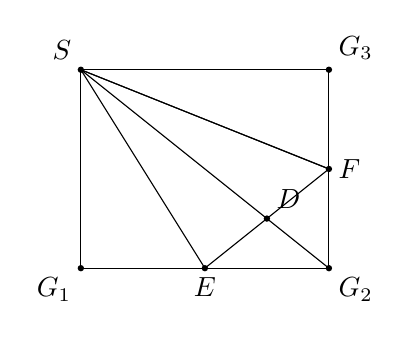
\begin{tikzpicture}[scale=1.05,>=stealth]
  \coordinate (S) at (0,2.4);
  \coordinate (G3) at (3,2.4);
  \coordinate (G2) at (3,0);
  \coordinate (G1) at (0,0);
  \coordinate (E) at (1.5,0);
  \coordinate (F) at (3,1.2);
  \coordinate (D) at (2.25,0.6);
  \draw (S)--(G3)--(G2)--(G1)--cycle;
  \draw (S)--(E)--(F)--cycle;
  \draw (S)--(F);
  \draw (S)--(G2);
  \draw (E)--(G2);
  \draw (F)--(G3);
  \fill (S) circle (1.1pt) node[above left] {$S$};
  \fill (G3) circle (1.1pt) node[above right] {$G_3$};
  \fill (G2) circle (1.1pt) node[below right] {$G_2$};
  \fill (G1) circle (1.1pt) node[below left] {$G_1$};
  \fill (E) circle (1.1pt) node[below] {$E$};
  \fill (F) circle (1.1pt) node[right] {$F$};
  \fill (D) circle (1.1pt) node[above right] {$D$};
\end{tikzpicture}
\end{center}
\nopagebreak[4]
（A）$SG\perp\triangle EFG$ 所在平面　　（B）$SD\perp\triangle EFG$ 所在平面

（C）$GF\perp\triangle SEF$ 所在平面　　（D）$GD\perp\triangle SEF$ 所在平面

\Needspace{4\baselineskip}
\textbf{解析}

\Needspace{5\baselineskip}
设正方形边长为 $2a$。折叠后

\nopagebreak[4]
\[
SG=2a,\ GE=GF=a,\ SE=SF=\sqrt5a.
\]

\Needspace{5\baselineskip}
于是

\nopagebreak[4]
\[
SG^2+GE^2=SE^2,
SG^2+GF^2=SF^2.
\]

\Needspace{5\baselineskip}
所以 $SG$ 同时垂直于 $GE\text{、}GF$。这两条直线在平面 $EFG$ 内相交，故

\nopagebreak[4]
\[
SG\perp\text{\text{平面} }EFG.
\]

选（A）。

\gkanswer{答案：A}

\end{answer}
\begin{answer}
\gksolhead{9}{}

\textbf{题目}：

在下列各图中，$y=ax^2+bx$ 与 $y=ax+b$（$ab\ne0$）的图象只可能是\mbox{（　　）}
\nopagebreak[4]
\begin{center}% 1986 年全国卷理科第 9 题：四个函数图象选项
\begin{tikzpicture}[scale=0.72,>=stealth]
  \foreach \dx/\dy/\lab/\curve/\line in {
    0/2.25/{（A）}/{1.55*(\x+0.45)^2-0.55}/{0.85*\x+0.55},
    3.15/2.25/{（B）}/{1.55*\x*\x-1.55*\x}/{-0.85*\x+0.80},
    0/0/{（C）}/{-1.45*\x*\x+1.45*\x}/{-0.72*\x+0.85},
    3.15/0/{（D）}/{-1.45*\x*\x+1.45*\x}/{0.72*\x-0.55}
  } {
    \begin{scope}[shift={(\dx,\dy)}]
      \draw[->] (-1.35,0)--(1.45,0) node[right] {$x$};
      \draw[->] (0,-1.35)--(0,1.45) node[above] {$y$};
      \draw[thick,domain=-1.15:1.15,samples=80]
        plot (\x,{\curve});
      \draw[thick,domain=-1.25:1.25]
        plot (\x,{\line});
      \node[below] at (0,-1.65) {\lab};
      \node[below left] at (0,0) {$O$};
    \end{scope}
  }
\end{tikzpicture}
\end{center}
\nopagebreak[4]
\Needspace{4\baselineskip}
\textbf{解析}

抛物线 $y=ax^2+bx=x(ax+b)$ 必过原点，另一个横截距为 $-b/a$；直线 $y=ax+b$ 的斜率为 $a$，也经过横截距 $-b/a$。同时，抛物线的开口方向由 $a$ 决定，必须与直线斜率的正负相容。四图中只有（C）满足这些条件。

\gkanswer{答案：C}

\end{answer}
\begin{answer}
\gksolhead{10}{}

\textbf{题目}：

当 $x\in[-1,0]$ 时，在下面关系式中正确的是\mbox{（　　）}

（A）$\pi-\arccos(-x)=\arcsin\sqrt{1-x^2}$

（B）$\pi-\arcsin(-x)=\arccos\sqrt{1-x^2}$

（C）$\pi-\arccos x=\arcsin\sqrt{1-x^2}$

（D）$\pi-\arcsin x=\arccos\sqrt{1-x^2}$

\Needspace{4\baselineskip}
\textbf{解析}

\Needspace{5\baselineskip}
当 $x\in[-1,0]$ 时，令 $x=-\sin\alpha$，其中 $0\le\alpha\le\pi/2$。则

\nopagebreak[4]
\[
\arccos x=\frac\pi2+\alpha,
\,
\arcsin\sqrt{1-x^2}
=\arcsin(\cos\alpha)
=\frac\pi2-\alpha.
\]

\Needspace{5\baselineskip}
因此

\nopagebreak[4]
\[
\pi-\arccos x=\arcsin\sqrt{1-x^2},
\]

故选（C）。

\gkanswer{答案：C}

\end{answer}
\begin{answer}
\gksolhead{11}{}

\textbf{题目}：

\Needspace{5\baselineskip}
求方程

\nopagebreak[4]
\[
\sqrt{25^{(x^2+x-0.5)}}=\sqrt[4]{5}
\]

的解。

\Needspace{4\baselineskip}
\textbf{解析}

\Needspace{5\baselineskip}
令 $t=x^2+x-\frac12$。则

\nopagebreak[4]
\[
\sqrt{25^t}=5^t,\
\sqrt[4]{5}=5^{1/4}.
\]

\Needspace{5\baselineskip}
所以

\nopagebreak[4]
\[
x^2+x-\frac12=\frac14
\Longrightarrow x^2+x-\frac34=0.
\]

\Needspace{5\baselineskip}
故

\nopagebreak[4]
\[
x=\frac12\ \text{\text{或}}\ x=-\frac32.
\]

\gkanswer{答案：$x=\dfrac12$ 或 $x=-\dfrac32$。}

\end{answer}
\begin{answer}
\gksolhead{12}{}

\textbf{题目}：

\Needspace{5\baselineskip}
已知

\nopagebreak[4]
\[
\omega=\frac{-1-\sqrt3i}{2},
\]

求 $\omega^2+\omega+1$ 的值。

\Needspace{4\baselineskip}
\textbf{解析}

\nopagebreak[4]
\[
\omega=-\frac12-\frac{\sqrt3}{2}i
\]

\Needspace{5\baselineskip}
是非实三次单位根，满足

\nopagebreak[4]
\[
\omega^2+\omega+1=0.
\]

\gkanswer{答案：$0$。}

\end{answer}
\begin{answer}
\gksolhead{13}{}

\textbf{题目}：

在 $xOy$ 平面上，四边形 $ABCD$ 的四个顶点坐标依次为 $(0,0)\text{、}(1,0)\text{、}(2,1)$ 及 $(0,3)$，求这个四边形绕 $x$ 轴旋转一周所得到的几何体的体积。

\Needspace{4\baselineskip}
\textbf{解析}

\Needspace{5\baselineskip}
对四边形作竖直截面。边 $CD$ 的方程为 $y=3-x$；在 $1\le x\le2$ 时，边 $BC$ 的方程为 $y=x-1$。旋转体体积为

\nopagebreak[4]
\[
\begin{aligned}
V
&=\pi\int_0^1(3-x)^2\,dx\\
&+\pi\int_1^2\left[(3-x)^2-(x-1)^2\right]dx\\
&=\pi\left(\frac{19}{3}+2\right)
=\frac{25\pi}{3}.
\end{aligned}
\]

\gkanswer{答案：$\dfrac{25\pi}{3}$。}

\end{answer}
\begin{answer}
\gksolhead{14}{}

\textbf{题目}：

\Needspace{5\baselineskip}
求

\nopagebreak[4]
\[
\lim_{n\to\infty}\frac{3^n+(-2)^n}{3^{n+1}+(-2)^{n+1}}.
\]

\Needspace{4\baselineskip}
\textbf{解析}

\Needspace{5\baselineskip}
同除以 $3^n$：

\nopagebreak[4]
\[
\lim_{n\to\infty}
\frac{1+\left(-\frac23\right)^n}
{3-2\left(-\frac23\right)^n}
=\frac13.
\]

\gkanswer{答案：$\dfrac13$。}

\end{answer}
\begin{answer}
\gksolhead{15}{}

\textbf{题目}：

\Needspace{5\baselineskip}
求

\nopagebreak[4]
\[
\left(2x^3-\frac1{x^2}\right)^5
\]

展开式中的常数项。

\Needspace{4\baselineskip}
\textbf{解析}

\Needspace{5\baselineskip}
通项

\nopagebreak[4]
\[
\binom5k(2x^3)^{5-k}\left(-\frac1{x^2}\right)^k
\]

\Needspace{5\baselineskip}
中的幂次为 $15-5k$。常数项要求 $k=3$，因此常数项为

\nopagebreak[4]
\[
\binom53 2^2(-1)^3=-40.
\]

\gkanswer{答案：$-40$。}

\end{answer}
\begin{answer}
\gksolhead{16}{}

\textbf{题目}：

已知 $\sin\theta-\cos\theta=\dfrac12$，求 $\sin^3\theta-\cos^3\theta$ 的值。

\Needspace{4\baselineskip}
\textbf{解析}

\Needspace{5\baselineskip}
由

\nopagebreak[4]
\[
(\sin\theta-\cos\theta)^2
=1-2\sin\theta\cos\theta
=\frac14
\]

\Needspace{5\baselineskip}
得

\nopagebreak[4]
\[
\sin\theta\cos\theta=\frac38.
\]

\Needspace{5\baselineskip}
于是

\nopagebreak[4]
\[
\begin{aligned}
\sin^3\theta-\cos^3\theta
&=(\sin\theta-\cos\theta)
(\sin^2\theta+\sin\theta\cos\theta+\cos^2\theta)\\
&=\frac12\left(1+\frac38\right)
=\frac{11}{16}.
\end{aligned}
\]

\gkanswer{答案：$\dfrac{11}{16}$。}

\end{answer}
\begin{answer}
\gksolhead{17}{}

\textbf{题目}：

如图，$AB$ 是圆 $O$ 的直径，$PA$ 垂直于圆 $O$ 所在的平面，$C$ 是圆周上不同于 $A\text{、}B$ 的任一点，求证：平面 $PAC$ 垂直于平面 $PBC$。
\nopagebreak[4]
\begin{center}% 1986 年全国卷理科第 17 题：圆的直径与三棱锥示意图
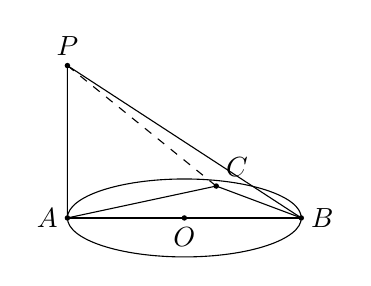
\begin{tikzpicture}[scale=0.9,>=stealth]
  \draw (0,0) ellipse (1.65 and 0.55);
  \draw[dashed] (-1.65,0)--(1.65,0);
  \draw (-1.65,0)--(1.65,0);
  \fill (0,0) circle (1.1pt) node[below] {$O$};
  \fill (-1.65,0) circle (1.1pt) node[left] {$A$};
  \fill (1.65,0) circle (1.1pt) node[right] {$B$};
  \coordinate (C) at (0.45,0.45);
  \fill (C) circle (1.1pt) node[above right] {$C$};
  \coordinate (P) at (-1.65,2.15);
  \fill (P) circle (1.1pt) node[above] {$P$};
  \draw (P)--(-1.65,0);
  \draw (P)--(1.65,0);
  \draw[dashed] (P)--(C);
  \draw (C)--(-1.65,0);
  \draw (C)--(1.65,0);
\end{tikzpicture}
\end{center}
\nopagebreak[4]
\Needspace{4\baselineskip}
\textbf{解析}

\Needspace{5\baselineskip}
由 $AB$ 是圆的直径，圆周角定理给出

\nopagebreak[4]
\[
\angle ACB=90^\circ,\ AC\perp BC.
\]

\Needspace{5\baselineskip}
又因 $PA$ 垂直于圆所在平面，而 $BC$ 在该平面内，所以 $PA\perp BC$。直线 $PA\text{、}AC$ 是平面 $PAC$ 内相交的两条直线，且 $BC$ 同时垂直于它们，因此

\nopagebreak[4]
\[
BC\perp\text{\text{平面} }PAC.
\]

\Needspace{5\baselineskip}
而 $BC$ 在平面 $PBC$ 内，故

\nopagebreak[4]
\[
\text{\text{平面} }PAC\perp\text{\text{平面} }PBC.
\]

\gkanswer{答案：$\text{\text{平面} }PAC\perp\text{\text{平面} }PBC$。}

\end{answer}
\begin{answer}
\gksolhead{18}{}

\textbf{题目}：

\Needspace{5\baselineskip}
当 $\sin2x>0$，求不等式

\nopagebreak[4]
\[
\log_{0.5}(x^2-2x-15)>\log_{0.5}(x+13)
\]

的解集。

\Needspace{4\baselineskip}
\textbf{解析}

\Needspace{5\baselineskip}
对数有意义要求

\nopagebreak[4]
\[
x^2-2x-15>0,\ x+13>0.
\]

\Needspace{5\baselineskip}
所以定义域为 $(-13,-3)\cup(5,+\infty)$。因底数 $0.5<1$，不等式反向：

\nopagebreak[4]
\[
x^2-2x-15<x+13
\Longrightarrow x^2-3x-28<0
\Longrightarrow -4<x<7.
\]

\Needspace{5\baselineskip}
与定义域合并得

\nopagebreak[4]
\[
(-4,-3)\cup(5,7).
\]

\Needspace{5\baselineskip}
再与

\nopagebreak[4]
\[
\sin2x>0
\Longleftrightarrow
x\in\left(k\pi,k\pi+\frac\pi2\right)
\]

\Needspace{5\baselineskip}
相交。由于 $-\pi\in(-4,-3)$ 且 $2\pi\in(5,7)$，最终解集为

\nopagebreak[4]
\[
(-\pi,-3)\cup(2\pi,7).
\]

\gkanswer{答案：$(-\pi,-3)\cup(2\pi,7)$。}

\end{answer}
\begin{answer}
\gksolhead{19}{}

\textbf{题目}：

如图，在平面直角坐标系中，在 $y$ 轴的正半轴（坐标原点除外）上给定两点 $A\text{、}B$ 试在 $x$ 轴的正半轴（坐标原点除外）上求点 $C$，使 $\angle ACB$ 取得最大值。
\nopagebreak[4]
\begin{center}% 1986 年全国卷理科第 19 题：最大角示意图
\begin{tikzpicture}[scale=0.95,>=stealth]
  \draw[->] (-0.2,0)--(4.0,0) node[right] {$x$};
  \draw[->] (0,-0.2)--(0,3.5) node[above] {$y$};
  \coordinate (A) at (0,3.0);
  \coordinate (B) at (0,1.45);
  \coordinate (C) at (2.1,0);
  \fill (A) circle (1.1pt) node[left] {$A$};
  \fill (B) circle (1.1pt) node[left] {$B$};
  \fill (C) circle (1.1pt) node[below] {$C$};
  \fill (0,0) circle (1.1pt) node[below left] {$O$};
  \draw (A)--(C)--(B);
\end{tikzpicture}
\end{center}
\nopagebreak[4]
\Needspace{4\baselineskip}
\textbf{解析}

\Needspace{5\baselineskip}
设 $A=(0,a)$、$B=(0,b)$，其中 $a>b>0$，$C=(t,0)$，$t>0$。角度为

\nopagebreak[4]
\[
\phi(t)=\arctan\frac at-\arctan\frac bt.
\]

\Needspace{5\baselineskip}
求导：

\nopagebreak[4]
\[
\phi'(t)
=-\frac a{t^2+a^2}+\frac b{t^2+b^2}
=\frac{(a-b)(ab-t^2)}
{(t^2+a^2)(t^2+b^2)}.
\]

\Needspace{5\baselineskip}
所以 $\phi$ 在 $0<t<\sqrt{ab}$ 上递增，在 $t>\sqrt{ab}$ 上递减，最大值在

\nopagebreak[4]
\[
t=\sqrt{ab}
\]

处取得。因此 $C=(\sqrt{ab},0)$。

\gkanswer{答案：若 $OA=a$、$OB=b$，则 $C=(\sqrt{ab},0)$。}

\end{answer}
\begin{answer}
\gksolhead{20}{}

\textbf{题目}：

已知集合 $A$ 和集合 $B$ 各含有 12 个元素，$A\cap B$ 含有 4 个元素，试求同时满足下面两个条件的集合 $C$ 的个数：

（1）$C\subseteq A\cup B$ 且 $C$ 中含有 3 个元素；

（2）$C\cap A\ne\varnothing$（$\varnothing$ 表示空集）。

\Needspace{4\baselineskip}
\textbf{解析}

独立公开资料均将本题题面记为 $|A|=|B|=12$、$|A\cap B|=4$，并给出答案 $1084$；这与固定源中 \texttt{A$\cup$B} 的显然矛盾相互印证。以下按交叉核定后的题面计算。

\Needspace{5\baselineskip}
由

\nopagebreak[4]
\[
|A\cup B|=|A|+|B|-|A\cap B|=12+12-4=20\text{。}
\]

\Needspace{5\baselineskip}
集合 $C$ 是 $A\cup B$ 的 3 元子集，且至少含有一个 $A$ 中的元素。因此可以从全部 3 元子集中排除完全取自 $(A\cup B)\setminus A$ 的情形。注意

\nopagebreak[4]
\[
|(A\cup B)\setminus A|=|B\setminus A|=20-12=8\text{，}
\]

\Needspace{5\baselineskip}
故

\nopagebreak[4]
\[
\binom{20}{3}-\binom{8}{3}=1140-56=1084\text{。}
\]

所以满足条件的集合 $C$ 有 $1084$ 个。

\gkanswer{答案：$1084$。}

\end{answer}
\begin{answer}
\gksolhead{21}{}

\textbf{题目}：

\Needspace{5\baselineskip}
过点 $M(-1,0)$ 的直线 $L_1$ 与抛物线

\nopagebreak[4]
\[
y^2=4x
\]

交于 $P_1\text{、}P_2$ 两点。记：线段 $P_1P_2$ 的中点为 $P$；过点 $P$ 和这个抛物线的焦点 $F$ 的直线为 $L_2$；$L_1$ 的斜率为 $k$。试把直线 $L_2$ 的斜率与直线 $L_1$ 的斜率之比表示为 $k$ 的函数，并指出这个函数的定义域、单调区间，同时说明在每一单调区间上它是增函数还是减函数。

\Needspace{4\baselineskip}
\textbf{解析}

\Needspace{5\baselineskip}
设直线 $L_1$ 的斜率为 $k$，用参数表示抛物线上的交点：

\nopagebreak[4]
\[
P_i=(t_i^2,2t_i)\ (i=1,2).
\]

\Needspace{5\baselineskip}
因为 $L_1$ 过 $M(-1,0)$，所以

\nopagebreak[4]
\[
2t_i=k(t_i^2+1),
\]

\Needspace{5\baselineskip}
即 $t_1,t_2$ 是方程

\nopagebreak[4]
\[
kt^2-2t+k=0
\]

\Needspace{5\baselineskip}
的两个根。于是

\nopagebreak[4]
\[
t_1+t_2=\frac2k,\ t_1t_2=1.
\]

\Needspace{5\baselineskip}
线段中点为

\nopagebreak[4]
\[
P=\left(\frac{t_1^2+t_2^2}{2},t_1+t_2\right)
=\left(\frac2{k^2}-1,\frac2k\right).
\]

\Needspace{5\baselineskip}
抛物线焦点为 $F=(1,0)$，故 $L_2$ 的斜率为

\nopagebreak[4]
\[
m_2=\frac{2/k}{2/k^2-2}
=\frac{k}{1-k^2}.
\]

\Needspace{5\baselineskip}
所以所求比值函数为

\nopagebreak[4]
\[
f(k)=\frac{m_2}{k}=\frac1{1-k^2}.
\]

\Needspace{5\baselineskip}
要有两个相异交点，判别式要求 $0<|k|<1$，故定义域为

\nopagebreak[4]
\[
(-1,0)\cup(0,1).
\]

\Needspace{5\baselineskip}
又

\nopagebreak[4]
\[
f'(k)=\frac{2k}{(1-k^2)^2},
\]

所以 $f$ 在 $(-1,0)$ 上递减，在 $(0,1)$ 上递增。

\gkanswer{答案：见解析正文。}

\end{answer}
\begin{answer}
\gksolhead{22}{}

\textbf{题目}：

\Needspace{5\baselineskip}
已知 $x_1>0$，$x_1\ne1$，且

\nopagebreak[4]
\[
x_{n+1}=\frac{x_n(x_n^2+3)}{3x_n^2+1},\ (n=1,2,\cdots).
\]

试证：数列 $\{x_n\}$ 或者对任意自然数 $n$ 都满足 $x_n<x_{n+1}$，或者对任意自然数 $n$ 都满足 $x_n>x_{n+1}$。

\Needspace{0.25\textheight}
\textbf{附加题}

\Needspace{4\baselineskip}
\textbf{解析}

\Needspace{5\baselineskip}
设

\nopagebreak[4]
\[
T(x)=\frac{x(x^2+3)}{3x^2+1}.
\]

\Needspace{5\baselineskip}
当 $x>0$ 时，$T(x)>0$。并且

\nopagebreak[4]
\[
T(x)-1
=\frac{x(x^2+3)-(3x^2+1)}{3x^2+1}
=\frac{(x-1)^3}{3x^2+1},
\]

所以 $x-1$ 的符号在迭代中保持不变。

\Needspace{5\baselineskip}
另一方面，

\nopagebreak[4]
\[
T(x)-x
=\frac{2x(1-x^2)}{3x^2+1}.
\]

若 $0<x_1<1$，则归纳得 $0<x_n<1$，从而 $x_{n+1}-x_n>0$，数列严格递增。若 $x_1>1$，则归纳得 $x_n>1$，从而 $x_{n+1}-x_n<0$，数列严格递减。这证明了题面所述二择一结论。

\gkanswer{答案：见解析正文。}

\end{answer}
\begin{answer}
\gksolhead{23}{}

\textbf{题目}：

\Needspace{5\baselineskip}
求

\nopagebreak[4]
\[
y=x\arctan x^2
\]

的导数。

\Needspace{4\baselineskip}
\textbf{解析}

\Needspace{5\baselineskip}
由乘积法则和链式法则，

\nopagebreak[4]
\[
y'=\arctan x^2+x\cdot\frac{2x}{1+x^4}
=\arctan x^2+\frac{2x^2}{1+x^4}.
\]

\gkanswer{答案：$y'=\arctan x^2+\dfrac{2x^2}{1+x^4}$。}

\end{answer}
\begin{answer}
\gksolhead{24}{}

\textbf{题目}：

\Needspace{5\baselineskip}
求过点 $(-1,0)$ 并与曲线

\nopagebreak[4]
\[
y=\frac{x+1}{x+2}
\]

相切的直线方程。

\Needspace{4\baselineskip}
\textbf{解析}

\Needspace{5\baselineskip}
设切点横坐标为 $t$，令

\nopagebreak[4]
\[
f(x)=\frac{x+1}{x+2},\ f'(x)=\frac1{(x+2)^2}.
\]

\Needspace{5\baselineskip}
切线过 $(-1,0)$，所以

\nopagebreak[4]
\[
0=f(t)+f'(t)(-1-t)
=\frac{(t+1)^2}{(t+2)^2}.
\]

\Needspace{5\baselineskip}
故 $t=-1$。切点为 $(-1,0)$，切线斜率为 $f'(-1)=1$，所求直线为

\nopagebreak[4]
\[
y=x+1.
\]

\gkanswer{答案：$y=x+1$。}

\end{answer}